\documentclass{standalone}
\usepackage{tikz}
\usetikzlibrary{patterns, positioning}


\begin{document}
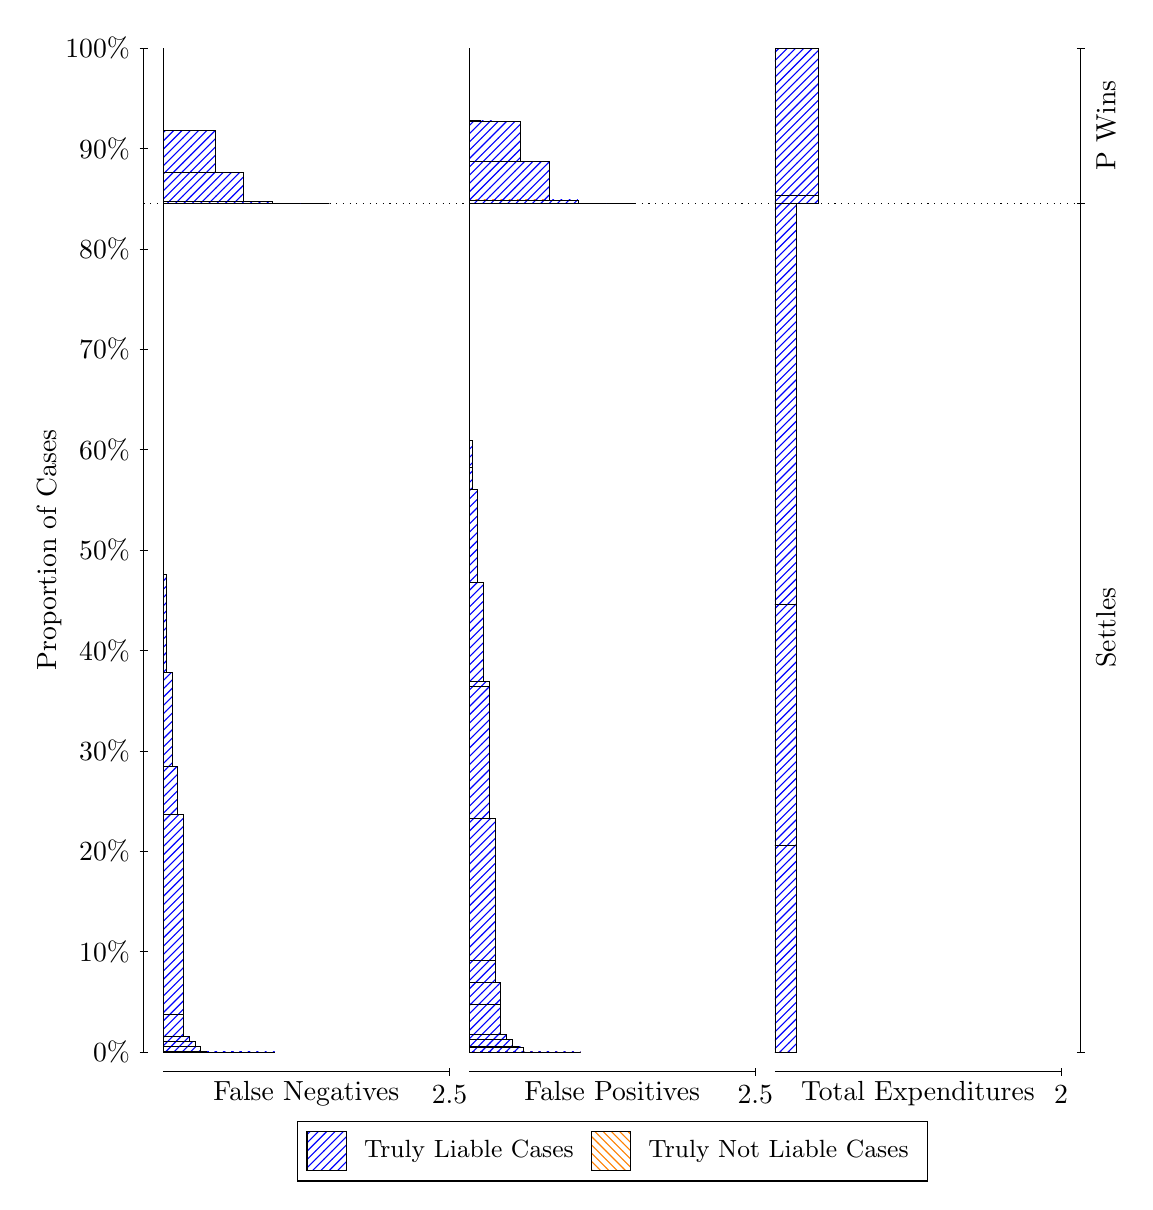
\begin{tikzpicture}
\draw[black, very thin] (1.5,1.75) -- (1.5,14.5);
\node[rotate=90, text=black, anchor=center] at (0.3, 8.125) {Proportion of Cases};
\draw[black, very thin] (1.45,1.75) -- (1.55,1.75);
\node[text=black, anchor=east] at (1.45, 1.75) {0\%};
\draw[black, very thin] (1.45,3.025) -- (1.55,3.025);
\node[text=black, anchor=east] at (1.45, 3.025) {10\%};
\draw[black, very thin] (1.45,4.3) -- (1.55,4.3);
\node[text=black, anchor=east] at (1.45, 4.3) {20\%};
\draw[black, very thin] (1.45,5.575) -- (1.55,5.575);
\node[text=black, anchor=east] at (1.45, 5.575) {30\%};
\draw[black, very thin] (1.45,6.85) -- (1.55,6.85);
\node[text=black, anchor=east] at (1.45, 6.85) {40\%};
\draw[black, very thin] (1.45,8.125) -- (1.55,8.125);
\node[text=black, anchor=east] at (1.45, 8.125) {50\%};
\draw[black, very thin] (1.45,9.4) -- (1.55,9.4);
\node[text=black, anchor=east] at (1.45, 9.4) {60\%};
\draw[black, very thin] (1.45,10.675) -- (1.55,10.675);
\node[text=black, anchor=east] at (1.45, 10.675) {70\%};
\draw[black, very thin] (1.45,11.95) -- (1.55,11.95);
\node[text=black, anchor=east] at (1.45, 11.95) {80\%};
\draw[black, very thin] (1.45,13.225) -- (1.55,13.225);
\node[text=black, anchor=east] at (1.45, 13.225) {90\%};
\draw[black, very thin] (1.45,14.5) -- (1.55,14.5);
\node[text=black, anchor=east] at (1.45, 14.5) {100\%};

\draw[black, very thin] (13.4,1.75) -- (13.4,14.5);
\draw[black, very thin] (13.35,1.75) -- (13.45,1.75);
\node[anchor=west] at (13.35, 1.75) {};
\draw[black, very thin] (13.35,12.531) -- (13.45,12.531);
\node[anchor=west] at (13.35, 12.531) {};
\draw[black, very thin] (13.35,14.5) -- (13.45,14.5);
\node[anchor=west] at (13.35, 14.5) {};

\draw[black, very thin, pattern color=blue, pattern=north east lines] (1.75,1.75) rectangle (3.167,1.75);
\draw[black, very thin, pattern color=blue, pattern=north east lines] (1.75,1.75) rectangle (3.0217,1.75);
\draw[black, very thin, pattern color=blue, pattern=north east lines] (1.75,1.75) rectangle (2.8763,1.75);
\draw[black, very thin, pattern color=blue, pattern=north east lines] (1.75,1.75) rectangle (2.8037,1.75);
\draw[black, very thin, pattern color=blue, pattern=north east lines] (1.75,1.75) rectangle (2.731,1.75);
\draw[black, very thin, pattern color=blue, pattern=north east lines] (1.75,1.75) rectangle (2.6583,1.75);
\draw[black, very thin, pattern color=blue, pattern=north east lines] (1.75,1.75) rectangle (2.5857,1.75);
\draw[black, very thin, pattern color=blue, pattern=north east lines] (1.75,1.75) rectangle (2.513,1.75);
\draw[black, very thin, pattern color=blue, pattern=north east lines] (1.75,1.75) rectangle (2.4403,1.75);
\draw[black, very thin, pattern color=blue, pattern=north east lines] (1.75,1.75) rectangle (2.3677,1.7506);
\draw[black, very thin, pattern color=blue, pattern=north east lines] (1.75,1.7506) rectangle (2.295,1.7552);
\draw[black, very thin, pattern color=blue, pattern=north east lines] (1.75,1.7552) rectangle (2.2223,1.8185);
\draw[black, very thin, pattern color=blue, pattern=north east lines] (1.75,1.8185) rectangle (2.1497,1.8839);
\draw[black, very thin, pattern color=blue, pattern=north east lines] (1.75,1.8839) rectangle (2.077,1.9501);
\draw[black, very thin, pattern color=blue, pattern=north east lines] (1.75,1.9501) rectangle (2.0043,2.2239);
\draw[black, very thin, pattern color=blue, pattern=north east lines] (1.75,2.2239) rectangle (2.0043,4.7657);
\draw[black, very thin, pattern color=blue, pattern=north east lines] (1.75,4.7657) rectangle (1.9317,5.3781);
\draw[black, very thin, pattern color=blue, pattern=north east lines] (1.75,5.3781) rectangle (1.859,6.5672);
\draw[black, very thin, pattern color=blue, pattern=north east lines] (1.75,6.5672) rectangle (1.7863,7.8221);
\draw[black, very thin, pattern color=orange, pattern=north west lines] (1.75,7.8221) rectangle (1.75,7.8221);
\draw[black, very thin, pattern color=blue, pattern=north east lines] (1.75,7.8221) rectangle (1.75,12.531);
\draw[black, very thin, pattern color=blue, pattern=north east lines] (1.75,12.531) rectangle (3.8573,12.531);
\draw[black, very thin, pattern color=blue, pattern=north east lines] (1.75,12.531) rectangle (3.494,12.531);
\draw[black, very thin, pattern color=blue, pattern=north east lines] (1.75,12.531) rectangle (3.1307,12.553);
\draw[black, very thin, pattern color=blue, pattern=north east lines] (1.75,12.553) rectangle (2.7673,12.918);
\draw[black, very thin, pattern color=blue, pattern=north east lines] (1.75,12.918) rectangle (2.622,12.918);
\draw[black, very thin, pattern color=blue, pattern=north east lines] (1.75,12.918) rectangle (2.404,13.454);
\draw[black, very thin, pattern color=blue, pattern=north east lines] (1.75,13.454) rectangle (2.2587,13.454);
\draw[black, very thin, pattern color=blue, pattern=north east lines] (1.75,13.454) rectangle (2.0407,13.455);
\draw[black, very thin, pattern color=blue, pattern=north east lines] (1.75,13.455) rectangle (1.8953,13.457);
\draw[black, very thin, pattern color=orange, pattern=north west lines] (1.75,13.457) rectangle (1.75,13.457);
\draw[black, very thin, pattern color=blue, pattern=north east lines] (1.75,13.457) rectangle (1.75,14.5);
\draw[black, very thin, pattern color=orange, pattern=north west lines] (5.6333,1.75) rectangle (7.0503,1.75);
\draw[black, very thin, pattern color=blue, pattern=north east lines] (5.6333,1.75) rectangle (7.0503,1.75);
\draw[black, very thin, pattern color=orange, pattern=north west lines] (5.6333,1.75) rectangle (6.7597,1.75);
\draw[black, very thin, pattern color=blue, pattern=north east lines] (5.6333,1.75) rectangle (6.7597,1.75);
\draw[black, very thin, pattern color=blue, pattern=north east lines] (5.6333,1.75) rectangle (6.687,1.75);
\draw[black, very thin, pattern color=orange, pattern=north west lines] (5.6333,1.75) rectangle (6.6143,1.75);
\draw[black, very thin, pattern color=blue, pattern=north east lines] (5.6333,1.75) rectangle (6.6143,1.75);
\draw[black, very thin, pattern color=orange, pattern=north west lines] (5.6333,1.75) rectangle (6.469,1.75);
\draw[black, very thin, pattern color=blue, pattern=north east lines] (5.6333,1.75) rectangle (6.469,1.75);
\draw[black, very thin, pattern color=blue, pattern=north east lines] (5.6333,1.75) rectangle (6.3963,1.7506);
\draw[black, very thin, pattern color=orange, pattern=north west lines] (5.6333,1.7506) rectangle (6.3237,1.7506);
\draw[black, very thin, pattern color=blue, pattern=north east lines] (5.6333,1.7506) rectangle (6.3237,1.7513);
\draw[black, very thin, pattern color=blue, pattern=north east lines] (5.6333,1.7513) rectangle (6.3237,1.8155);
\draw[black, very thin, pattern color=blue, pattern=north east lines] (5.6333,1.8155) rectangle (6.251,1.8179);
\draw[black, very thin, pattern color=orange, pattern=north west lines] (5.6333,1.8179) rectangle (6.1783,1.8179);
\draw[black, very thin, pattern color=blue, pattern=north east lines] (5.6333,1.8179) rectangle (6.1783,1.9103);
\draw[black, very thin, pattern color=blue, pattern=north east lines] (5.6333,1.9103) rectangle (6.1057,1.9741);
\draw[black, very thin, pattern color=orange, pattern=north west lines] (5.6333,1.9741) rectangle (6.033,1.9741);
\draw[black, very thin, pattern color=blue, pattern=north east lines] (5.6333,1.9741) rectangle (6.033,2.361);
\draw[black, very thin, pattern color=blue, pattern=north east lines] (5.6333,2.361) rectangle (6.033,2.6372);
\draw[black, very thin, pattern color=blue, pattern=north east lines] (5.6333,2.6372) rectangle (5.9603,2.9118);
\draw[black, very thin, pattern color=blue, pattern=north east lines] (5.6333,2.9118) rectangle (5.9603,4.7159);
\draw[black, very thin, pattern color=orange, pattern=north west lines] (5.6333,4.7159) rectangle (5.8877,4.7159);
\draw[black, very thin, pattern color=blue, pattern=north east lines] (5.6333,4.7159) rectangle (5.8877,6.3949);
\draw[black, very thin, pattern color=blue, pattern=north east lines] (5.6333,6.3949) rectangle (5.8877,6.4585);
\draw[black, very thin, pattern color=blue, pattern=north east lines] (5.6333,6.4585) rectangle (5.815,7.7135);
\draw[black, very thin, pattern color=blue, pattern=north east lines] (5.6333,7.7135) rectangle (5.7423,8.9025);
\draw[black, very thin, pattern color=blue, pattern=north east lines] (5.6333,8.9025) rectangle (5.6697,9.1771);
\draw[black, very thin, pattern color=blue, pattern=north east lines] (5.6333,9.1771) rectangle (5.6697,9.515);
\draw[black, very thin, pattern color=blue, pattern=north east lines] (5.6333,9.515) rectangle (5.6333,12.531);
\draw[black, very thin, pattern color=orange, pattern=north west lines] (5.6333,12.531) rectangle (7.7407,12.531);
\draw[black, very thin, pattern color=blue, pattern=north east lines] (5.6333,12.531) rectangle (7.7407,12.531);
\draw[black, very thin, pattern color=orange, pattern=north west lines] (5.6333,12.531) rectangle (7.3773,12.531);
\draw[black, very thin, pattern color=blue, pattern=north east lines] (5.6333,12.531) rectangle (7.3773,12.531);
\draw[black, very thin, pattern color=orange, pattern=north west lines] (5.6333,12.531) rectangle (7.014,12.531);
\draw[black, very thin, pattern color=blue, pattern=north east lines] (5.6333,12.531) rectangle (7.014,12.571);
\draw[black, very thin, pattern color=orange, pattern=north west lines] (5.6333,12.571) rectangle (6.6507,12.571);
\draw[black, very thin, pattern color=blue, pattern=north east lines] (5.6333,12.571) rectangle (6.6507,13.057);
\draw[black, very thin, pattern color=blue, pattern=north east lines] (5.6333,13.057) rectangle (6.2873,13.573);
\draw[black, very thin, pattern color=orange, pattern=north west lines] (5.6333,13.573) rectangle (6.142,13.573);
\draw[black, very thin, pattern color=blue, pattern=north east lines] (5.6333,13.573) rectangle (6.142,13.573);
\draw[black, very thin, pattern color=blue, pattern=north east lines] (5.6333,13.573) rectangle (5.924,13.576);
\draw[black, very thin, pattern color=orange, pattern=north west lines] (5.6333,13.576) rectangle (5.7787,13.576);
\draw[black, very thin, pattern color=blue, pattern=north east lines] (5.6333,13.576) rectangle (5.7787,13.576);
\draw[black, very thin, pattern color=blue, pattern=north east lines] (5.6333,13.576) rectangle (5.7787,13.577);
\draw[black, very thin, pattern color=orange, pattern=north west lines] (5.6333,13.577) rectangle (5.6333,13.577);
\draw[black, very thin, pattern color=blue, pattern=north east lines] (5.6333,13.577) rectangle (5.6333,14.5);
\draw[black, very thin, pattern color=orange, pattern=north west lines] (9.5167,1.75) rectangle (9.7892,1.75);
\draw[black, very thin, pattern color=blue, pattern=north east lines] (9.5167,1.75) rectangle (9.7892,4.3746);
\draw[black, very thin, pattern color=orange, pattern=north west lines] (9.5167,4.3746) rectangle (9.7892,4.3746);
\draw[black, very thin, pattern color=blue, pattern=north east lines] (9.5167,4.3746) rectangle (9.7892,7.433);
\draw[black, very thin, pattern color=orange, pattern=north west lines] (9.5167,7.433) rectangle (9.7892,7.433);
\draw[black, very thin, pattern color=blue, pattern=north east lines] (9.5167,7.433) rectangle (9.7892,12.531);
\draw[black, very thin, pattern color=orange, pattern=north west lines] (9.5167,12.531) rectangle (10.062,12.531);
\draw[black, very thin, pattern color=blue, pattern=north east lines] (9.5167,12.531) rectangle (10.062,12.628);
\draw[black, very thin, pattern color=orange, pattern=north west lines] (9.5167,12.628) rectangle (10.062,12.628);
\draw[black, very thin, pattern color=blue, pattern=north east lines] (9.5167,12.628) rectangle (10.062,14.5);
\draw[black, dotted] (1.5,12.531) -- (13.4,12.531);
\draw[black, very thin] (1.75,1.5) -- (5.3833,1.5);
\node[text=black, anchor=north] at (3.5667, 1.5) {False Negatives};
\draw[black, very thin] (5.3833,1.45) -- (5.3833,1.55);
\node[text=black, anchor=north] at (5.3833, 1.45) {2.5};

\draw[black, very thin] (5.6333,1.5) -- (9.2667,1.5);
\node[text=black, anchor=north] at (7.45, 1.5) {False Positives};
\draw[black, very thin] (9.2667,1.45) -- (9.2667,1.55);
\node[text=black, anchor=north] at (9.2667, 1.45) {2.5};

\draw[black, very thin] (9.5167,1.5) -- (13.15,1.5);
\node[text=black, anchor=north] at (11.333, 1.5) {Total Expenditures};
\draw[black, very thin] (13.15,1.45) -- (13.15,1.55);
\node[text=black, anchor=north] at (13.15, 1.45) {2};

\node[text=black, centered, rotate=90] at (13.72, 7.1403) {Settles};
\node[text=black, centered, rotate=90] at (13.72, 13.515) {P Wins};

\draw (7.449999999999999,1.5) node[draw=none] (baseCoordinate) {};
\begin{scope}[align=center]
        \matrix[scale=0.5, draw=black, below=0.5cm of baseCoordinate, nodes={draw}, column sep=0.1cm]{
            \node[rectangle, draw, minimum width=0.5cm, minimum height=0.5cm, pattern color=blue, pattern=north east lines] {}; &
            \node[draw=none, font=\small, text=black] (B) {Truly Liable Cases}; &
            \node[rectangle, draw, minimum width=0.5cm, minimum height=0.5cm, pattern color=orange, pattern=north west lines] {}; &
            \node[draw=none, font=\small, text=black] (B) {Truly Not Liable Cases}; \\
            };
\end{scope}

\end{tikzpicture}
\end{document}